Sean $\ket\psi=\alpha\ket0+\beta\ket1$ y una solución del punto 1.3,
\[
  \ket{\psi'}=\alpha'\ket0+\beta'\ket1=e^{-i\eta}\bigl(-\alpha\ket0+e^{i\tau}\beta\ket1\bigr)
  \quad\eqref{eq:13-soluciones},
\]
que tiene las mismas probabilidades de medición que $\ket\psi$: $|\alpha'|=|\alpha|$ y
$|\beta'|=|\beta|$. En el punto 1.3 se sumaron los kets; en este punto se suman sus proyectores,
que primero se escriben como matrices.

\begin{definicionT}[Bra y proyector de un estado]
Al ket $\ket\psi=\alpha\ket0+\beta\ket1$ se le asocia la matriz columna de sus coordenadas en la
base $\{\ket0,\ket1\}$, y su \emph{bra} $\bra\psi$ es la matriz fila que se obtiene al trasponer
y conjugar esa columna:
\[
  \ket\psi=\begin{pmatrix}\alpha\\ \beta\end{pmatrix},\qquad
  \bra\psi=\begin{pmatrix}\overline\alpha & \overline\beta\end{pmatrix},
\]
donde $\overline z$ es el conjugado de $z$. El \emph{proyector} del estado es el producto de la
columna por la fila,
\begin{equation}\label{eq:14-proyector}
  \rho=\ket\psi\bra\psi
  =\begin{pmatrix}\alpha\\ \beta\end{pmatrix}
   \begin{pmatrix}\overline\alpha & \overline\beta\end{pmatrix}
  =\begin{pmatrix}\alpha\overline\alpha & \alpha\overline\beta\\
                  \beta\overline\alpha & \beta\overline\beta\end{pmatrix}
  =\begin{pmatrix}|\alpha|^2 & \alpha\overline\beta\\
                  \beta\overline\alpha & |\beta|^2\end{pmatrix},
\end{equation}
donde se usó $z\overline z=|z|^2$. Las filas y columnas de $\rho$ se numeran $0$ y $1$, como los
estados de la base, y su entrada en la fila $j$ y la columna $k$ se escribe $\rho_{jk}$.
\end{definicionT}

En la diagonal de $\rho$ están las probabilidades de medición de $\ket\psi$: $\rho_{00}=|\alpha|^2$
es la probabilidad de obtener $0$ y $\rho_{11}=|\beta|^2$ la de obtener $1$. Las fases de $\alpha$
y $\beta$ solo aparecen fuera de la diagonal.

\begin{definicionT}[Estado mixto]
Si $\rho_1,\dots,\rho_n$ son proyectores de estados puros y $p_1,\dots,p_n$ son números reales
con $p_i\ge0$ y $p_1+\dots+p_n=1$, la matriz
\[
  p_1\rho_1+\dots+p_n\rho_n
\]
es un \emph{estado mixto}. Representa un estado probabilístico: el sistema está en el estado
puro de $\rho_i$ con probabilidad $p_i$.
\end{definicionT}

El estado que se estudia en este punto es la mezcla de dos estados,
\begin{equation}\label{eq:14-mezcla}
  \rho_p=p\rho+(1-p)\rho',\qquad \rho=\ket\psi\bra\psi,\quad \rho'=\ket{\psi'}\bra{\psi'},
  \quad p\in[0,1],
\end{equation}
que está en $\ket\psi$ con probabilidad $p$ y en $\ket{\psi'}$ con probabilidad $1-p$.

%======================================================================
\subsection*{Las probabilidades de medición de la mezcla}
%======================================================================

Como la mezcla está en $\ket\psi$ con probabilidad $p$ y en $\ket{\psi'}$ con probabilidad $1-p$,
por la ley de probabilidad total la probabilidad de obtener $0$ es
\[
  P_{\rho_p}(0)=p\,P_\psi(0)+(1-p)\,P_{\psi'}(0)=p\,|\alpha|^2+(1-p)\,|\alpha'|^2
  =p\,|\alpha|^2+(1-p)\,|\alpha|^2=|\alpha|^2 ,
\]
donde se usó $|\alpha'|=|\alpha|$ y $p+(1-p)=1$. Del mismo modo, $P_{\rho_p}(1)=|\beta|^2$. Por tanto,
\[
  \destacado{P_{\rho_p}(0)=|\alpha|^2=P_\psi(0),\qquad P_{\rho_p}(1)=|\beta|^2=P_\psi(1),
  \qquad\text{para todo }p\in[0,1],}
\]
es decir, toda mezcla $p\rho+(1-p)\rho'$ tiene las mismas probabilidades de medición en la base
computacional que $\ket\psi$.

La misma cuenta se ve en las matrices. Por $\rho=\begin{pmatrix}|\alpha|^2 & \alpha\overline\beta\\ \beta\overline\alpha & |\beta|^2\end{pmatrix}$ \eqref{eq:14-proyector}, y como $|\alpha'|=|\alpha|$ y
$|\beta'|=|\beta|$, las matrices $\rho$ y $\rho'$ tienen la misma diagonal, $|\alpha|^2$ y
$|\beta|^2$. Como las matrices se suman y se multiplican por números entrada por entrada,
\begin{equation}\label{eq:14-rho-p}
  \rho_p=\begin{pmatrix}
     |\alpha|^2 & p\,\alpha\overline\beta+(1-p)\,\alpha'\overline{\beta'}\\[2pt]
     p\,\beta\overline\alpha+(1-p)\,\beta'\overline{\alpha'} & |\beta|^2
   \end{pmatrix}.
\end{equation}
La diagonal de $\rho_p$ son las probabilidades de $\ket\psi$ para todo $p$; el número $p$ solo
cambia las entradas de fuera de la diagonal.

\paragraph{Diferencia entre superponer y mezclar.} En el punto 1.3 se sumaron amplitudes, que son
números complejos con fase y se pueden anular: $\alpha+e^{i\eta}\alpha'=0$, y el resultado $0$
desaparece. En una mezcla se suman probabilidades, que son números reales no negativos y no se
anulan: $p|\alpha|^2+(1-p)|\alpha|^2=|\alpha|^2$. Por eso la superposición cambia las
probabilidades y la mezcla no.

%======================================================================
\subsection*{Interpretación en la esfera de Bloch}
%======================================================================

En el punto 1.2 se obtuvo el punto de un estado puro,
$\vec r=\bigl(2\Real(\overline\alpha\beta),\ 2\Imag(\overline\alpha\beta),\ A^2-B^2\bigr)$
\eqref{eq:a-c}. En la matriz $\rho$ se tiene $\rho_{00}=A^2$, $\rho_{11}=B^2$ y
$\rho_{10}=\beta\overline\alpha=\overline\alpha\beta$, así que el punto se lee de las entradas de
la matriz:
\begin{equation}\label{eq:14-bloch-matriz}
  \destacado{r_x=2\,\Real\rho_{10},\qquad
  r_y=2\,\Imag\rho_{10},\qquad
  r_z=\rho_{00}-\rho_{11}.}
\end{equation}
Para un estado mixto se usan las mismas fórmulas con las entradas de $\rho_p$. Como cada entrada
de $\rho_p$ es $p$ por la entrada de $\rho$ más $(1-p)$ por la de $\rho'$, si $\vec r$ y
$\vec r\,'$ son los puntos de $\ket\psi$ y $\ket{\psi'}$,
\begin{equation}\label{eq:14-segmento}
  \destacado{\vec r_p=p\,\vec r+(1-p)\,\vec r\,' ,\qquad p\in[0,1].}
\end{equation}

\begin{definicionT}[Cuerda]
Una \emph{cuerda} de la esfera es el segmento de recta que une dos puntos de su superficie. Sus
puntos, salvo los dos extremos, están en el interior de la esfera.
\end{definicionT}

Por $\vec r_p=p\,\vec r+(1-p)\,\vec r\,'$ \eqref{eq:14-segmento}, con $p=0$ se obtiene
$\vec r\,'$, con $p=1$ se obtiene $\vec r$, y con los valores intermedios se obtienen los puntos
del segmento que los une, más cerca de $\ket\psi$ cuanto mayor es $p$. Es decir, las mezclas
forman la cuerda que une $\ket{\psi'}$ con $\ket\psi$, y por eso quedan dentro de la esfera.
Además, todas tienen la misma altura, $r_z=\rho_{00}-\rho_{11}=|\alpha|^2-|\beta|^2$, porque la
diagonal de $\rho_p$ no depende de $p$. La cuerda es horizontal: une dos puntos del paralelo de
$\ket\psi$ del punto 1.3. Como $\rho_{00}+\rho_{11}=1$ y $\rho_{00}-\rho_{11}=r_z$, las
probabilidades solo dependen de la altura,
\[
  P(0)=\rho_{00}=\frac{1+r_z}{2},\qquad P(1)=\rho_{11}=\frac{1-r_z}{2},
\]
así que todos los puntos de la cuerda tienen las mismas probabilidades que $\ket\psi$. En resumen,
superponer $\ket\psi$ y $\ket{\psi'}$ (punto 1.3) lleva el estado al polo sur, mientras que
mezclarlos lo deja en la cuerda entre los dos, dentro de la esfera y a la misma altura.

%======================================================================
\subsection*{Comprobación con el ejemplo del punto 1.3}
%======================================================================

Se toma el ejemplo del punto 1.3, $\ket\psi=\frac{\sqrt3}{2}\ket0+\frac{i}{2}\ket1$, es decir,
$\alpha=\frac{\sqrt3}{2}$ y $\beta=\frac{i}{2}$, y la solución con $\tau=0$ y $\eta=0$,
$\ket{\psi'}=-\frac{\sqrt3}{2}\ket0+\frac{i}{2}\ket1$, es decir, $\alpha'=-\frac{\sqrt3}{2}$ y
$\beta'=\frac{i}{2}$.

\paragraph{Proyectores.} Como el conjugado de $\frac{i}{2}$ es $-\frac{i}{2}$, por
$\rho=\begin{pmatrix}|\alpha|^2 & \alpha\overline\beta\\ \beta\overline\alpha & |\beta|^2\end{pmatrix}$ \eqref{eq:14-proyector} las entradas de $\rho$ son
\[
  \rho_{00}=\tfrac34,\qquad
  \rho_{01}=\tfrac{\sqrt3}{2}\bigl(-\tfrac{i}{2}\bigr)=-\tfrac{\sqrt3}{4}i,\qquad
  \rho_{10}=\tfrac{i}{2}\cdot\tfrac{\sqrt3}{2}=\tfrac{\sqrt3}{4}i,\qquad
  \rho_{11}=\tfrac14 .
\]
En $\rho'$ solo cambia el signo de $\alpha$, así que la diagonal es la misma y cambia el signo de
las otras dos entradas: $\rho'_{01}=\bigl(-\tfrac{\sqrt3}{2}\bigr)\bigl(-\tfrac{i}{2}\bigr)=\tfrac{\sqrt3}{4}i$ y
$\rho'_{10}=\tfrac{i}{2}\bigl(-\tfrac{\sqrt3}{2}\bigr)=-\tfrac{\sqrt3}{4}i$. Entonces
\[
  \rho=\begin{pmatrix}\frac34 & -\frac{\sqrt3}{4}i\\[3pt] \frac{\sqrt3}{4}i & \frac14\end{pmatrix},
  \qquad
  \rho'=\begin{pmatrix}\frac34 & \frac{\sqrt3}{4}i\\[3pt] -\frac{\sqrt3}{4}i & \frac14\end{pmatrix}.
\]

\paragraph{Mezcla.} Al calcular $p\rho+(1-p)\rho'$ entrada por entrada, la diagonal queda
$p\cdot\frac34+(1-p)\cdot\frac34=\frac34$ y $p\cdot\frac14+(1-p)\cdot\frac14=\frac14$, y
\[
  (\rho_p)_{10}=p\cdot\tfrac{\sqrt3}{4}i+(1-p)\bigl(-\tfrac{\sqrt3}{4}i\bigr)=(2p-1)\tfrac{\sqrt3}{4}i ,
\]
y $(\rho_p)_{01}$ es su conjugado. Por tanto
\[
  \rho_p=\begin{pmatrix}\frac34 & -(2p-1)\frac{\sqrt3}{4}i\\[3pt]
                        (2p-1)\frac{\sqrt3}{4}i & \frac14\end{pmatrix}.
\]
Por ejemplo, con $p=\frac14$ se tiene $2p-1=-\frac12$, y
$\rho_{1/4}=\begin{pmatrix}\frac34 & \frac{\sqrt3}{8}i\\[2pt] -\frac{\sqrt3}{8}i & \frac14\end{pmatrix}$.

\paragraph{Probabilidades.} La diagonal no depende de $p$: para toda mezcla, $P(0)=\frac34$ y
$P(1)=\frac14$, que son las probabilidades de $\ket\psi$, pues $|\alpha|^2=\frac34$ y
$|\beta|^2=\frac14$. Esto comprueba en el ejemplo el resultado general; en el punto 1.5 se
comprueba también con mediciones simuladas.

\paragraph{Punto en la esfera.} El número $(\rho_p)_{10}=(2p-1)\frac{\sqrt3}{4}i$ tiene parte real
$0$ y parte imaginaria $(2p-1)\frac{\sqrt3}{4}$. Por
$r_x=2\,\Real\rho_{10},\ r_y=2\,\Imag\rho_{10},\ r_z=\rho_{00}-\rho_{11}$ \eqref{eq:14-bloch-matriz},
\[
  \vec r_p=\Bigl(0,\ (2p-1)\tfrac{\sqrt3}{2},\ \tfrac34-\tfrac14\Bigr)
          =\Bigl(0,\ (2p-1)\tfrac{\sqrt3}{2},\ \tfrac12\Bigr).
\]
\begin{center}
\renewcommand{\arraystretch}{1.45}
\begin{tabular}{cccc}
  $p$ & $\vec r_p$ & $P(0)$ & $P(1)$\\\hline
  $0$ & $\bigl(0,-\frac{\sqrt3}{2},\frac12\bigr)$, punto de $\ket{\psi'}$ & $\frac34$ & $\frac14$\\
  $\frac14$ & $\bigl(0,-\frac{\sqrt3}{4},\frac12\bigr)$ & $\frac34$ & $\frac14$\\
  $\frac12$ & $\bigl(0,0,\frac12\bigr)$, sobre el eje $z$ & $\frac34$ & $\frac14$\\
  $\frac34$ & $\bigl(0,\frac{\sqrt3}{4},\frac12\bigr)$ & $\frac34$ & $\frac14$\\
  $1$ & $\bigl(0,\frac{\sqrt3}{2},\frac12\bigr)$, punto de $\ket{\psi}$ & $\frac34$ & $\frac14$
\end{tabular}
\end{center}
Con $p=0$ y $p=1$ se obtienen los puntos de $\ket{\psi'}$ y de $\ket\psi$,
$(0,-0.866,0.5)$ y $(0,0.866,0.5)$, que son los que muestra el widget. Los demás están en la
cuerda que los une, a altura $\frac12$. Como en este caso $\ket{\psi'}$ está enfrente de
$\ket\psi$ en el paralelo, la cuerda pasa por el eje $z$, en $p=\frac12$ (figura~\ref{fig:14-bloch},
izquierda).

Con la solución de $\tau=\frac\pi2$ del punto 1.3, $\ket{\psi'}=-\frac{\sqrt3}{2}\ket0-\frac12\ket1$,
se tiene $\rho'_{10}=\bigl(-\frac12\bigr)\bigl(-\frac{\sqrt3}{2}\bigr)=\frac{\sqrt3}{4}$, así que
$(\rho_p)_{10}=p\frac{\sqrt3}{4}i+(1-p)\frac{\sqrt3}{4}$ y
\[
  \vec r_p=\Bigl((1-p)\tfrac{\sqrt3}{2},\ p\,\tfrac{\sqrt3}{2},\ \tfrac12\Bigr),
\]
que es otra cuerda del mismo paralelo, entre $(0.866,0,0.5)$ y $(0,0.866,0.5)$
(figura~\ref{fig:14-bloch}, derecha).

\begin{figure}[H]
\centering
\begin{minipage}{0.42\linewidth}\centering
  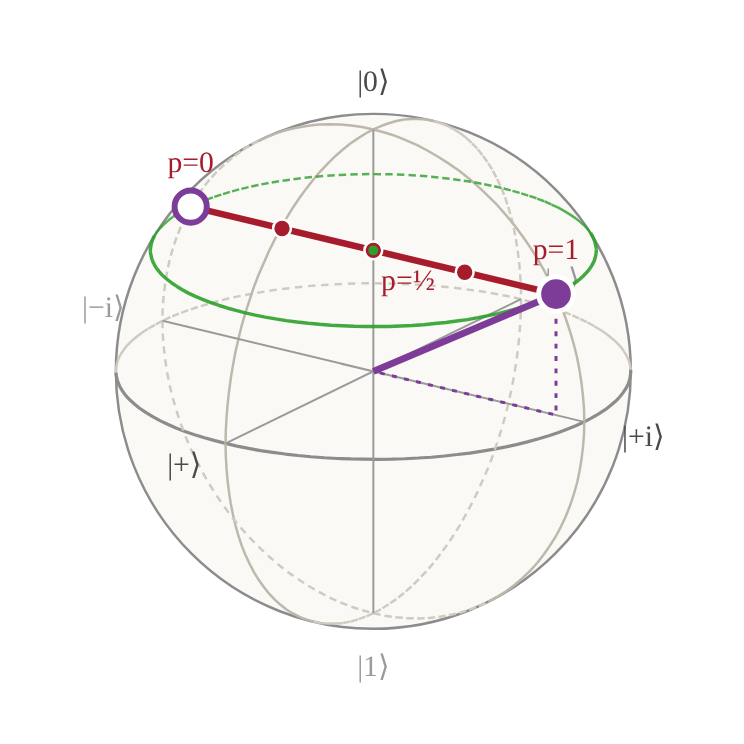
\includegraphics[width=\linewidth]{Imágenes/p14_mezcla_tau0.png}\\
  {\footnotesize $\ket{\psi'}$ con $\tau=0$}
\end{minipage}\hspace{0.06\linewidth}
\begin{minipage}{0.42\linewidth}\centering
  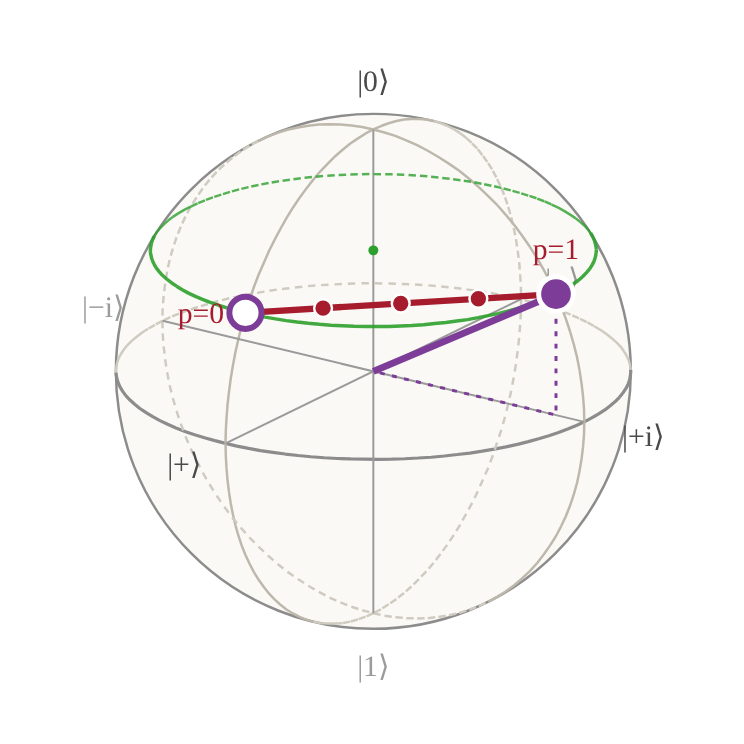
\includegraphics[width=\linewidth]{Imágenes/p14_mezcla_taupi2.png}\\
  {\footnotesize $\ket{\psi'}$ con $\tau=\frac\pi2$}
\end{minipage}
\caption{Panel (c) del widget con el estado $\ket\psi$ (punto morado relleno). Sobre la captura
se marcaron, con las coordenadas calculadas arriba, el punto de $\ket{\psi'}$ (círculo morado
vacío), el paralelo de altura $\frac12$ (verde) y los estados mixtos $\rho_p$ para
$p=0,\frac14,\frac12,\frac34,1$ (rojo). Las mezclas forman la cuerda que une $\ket{\psi'}$
($p=0$) con $\ket\psi$ ($p=1$), dentro de la esfera y a la misma altura.}
\label{fig:14-bloch}
\end{figure}
